% !TeX program = pdflatex
\documentclass[tikz,border=8pt]{standalone}
\usepackage{tikz}
\usetikzlibrary{angles,quotes,positioning,calc}
\definecolor{FigureBlue}{HTML}{2563EB}
\definecolor{FigureOrange}{HTML}{EA580C}
\definecolor{FigureSlate}{HTML}{64748B}
\begin{document}
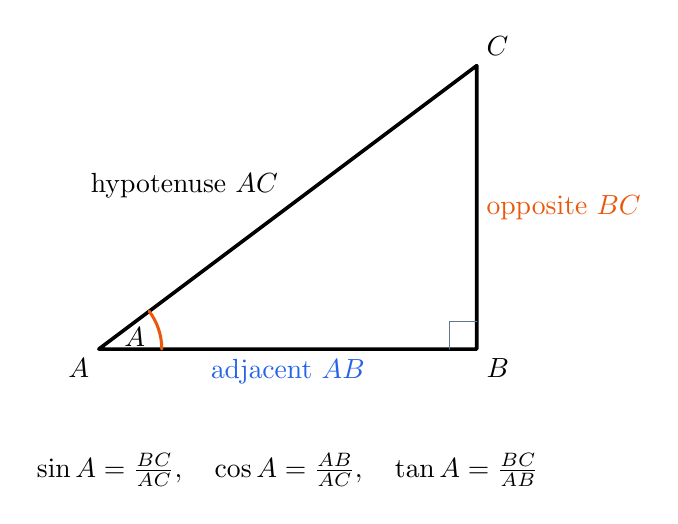
\begin{tikzpicture}[line cap=round,line join=round]
  \coordinate (A) at (0,0);\coordinate (B) at (4.8,0);\coordinate (C) at (4.8,3.6);
  \draw[line width=1.3pt] (A)--(B)--(C)--cycle;
  \draw[FigureSlate] (4.45,0)--(4.45,.35)--(4.8,.35);
  \pic[draw=FigureOrange,line width=1.1pt,angle radius=8mm,"$A$"] {angle=B--A--C};
  \node[below left] at (A) {$A$};\node[below right] at (B) {$B$};\node[above right] at (C) {$C$};
  \node[below,text=FigureBlue] at ($(A)!.5!(B)$) {adjacent $AB$};
  \node[right,text=FigureOrange] at ($(B)!.5!(C)$) {opposite $BC$};
  \node[above left] at ($(A)!.5!(C)$) {hypotenuse $AC$};
  \node[below=12mm] at ($(A)!.5!(B)$) {$\sin A=\frac{BC}{AC},\quad\cos A=\frac{AB}{AC},\quad\tan A=\frac{BC}{AB}$};
\end{tikzpicture}
\end{document}
